\section{Understanding the landscape}
\label{sec:landscape}
Before diving into our attack, we need to first improve our understanding of
DNS's role in Tor.  We begin by investigating how common it is for adversaries
to be able to observe DNS request but \emph{not} subsequent TCP connections of
Tor users (see Section~\ref{sec:as-exposure}).  We then seek to understand how
these results connect to the Tor network by determining the DNS resolvers used
by exit relays (see Section~\ref{sec:mapping-resolvers}).

\subsection{Measuring AS exposure of DNS queries}
\label{sec:as-exposure}
Adversaries that can observe both DNS and subsequent TCP traffic (e.g., the ISP
of an exit relay) can readily ignore DNS as traditional, TCP-based correlation
attacks work just fine~\cite{Murdoch2007a}.  But in this work, we consider
adversaries that can observe traffic entering the Tor network and \emph{some}
DNS requests exiting the network, e.g., requests addressed to DNS root servers.
But how common is this scenario?  How many adversaries are in a position to
observe DNS requests but not subsequent TCP connections?  We answer this
question by determining the number of ASs that DNS queries traverse versus the
number of ASs subsequent web traffic traverses.

We quantify the exposure of DNS versus web traffic as follows.  We begin with
Alexa's Top 1,000~\cite{alexatop1k}, a list of the 1,000 most popular web sites
as seen by the Alexa search engine.  For each site, we conducted two
experiments.  First, we ran a TCP traceroute to the site, targeting port 80 to
mimic web traffic.  Second, we determined the site's DNS delegation path using
the dig command's \texttt{+trace} feature.  The delegation path of a domain
name, say www.example.com, is a list of authoritative DNS servers, e.g., the
authoritative server for .com pointing to the authoritative server of
example.com, pointing to the authoritative server responsible for
www.example.com.  We ran UDP traceroutes to each server in the delegation path,
targeting port 53 to mimic DNS resolution.

For both experiments, we then mapped all IP addresses in the traceroutes to AS
numbers~\cite{ipasn}, and generated a set of traversed ASs for DNS traceroutes
($\mathcal{D}$), and a set of traversed ASs for web traceroutes
($\mathcal{W}$).  Having determined these two sets for each of Alexa's Top
1,000, we are now interested in the fraction of ASs that are \emph{only}
traversed for DNS traffic, but \emph{not} for web traffic.  To this end, we
define an exposure metric $\lambda$, defined as

\begin{equation}
\label{equ:exposure}
\lambda \in [0, 1] =
\frac{|\mathcal{D} \setminus \mathcal{W}|}
     {|\mathcal{D} \cup \mathcal{W}|}.
\end{equation}

The metric approaches 1 as the number of ASs that are only traversed for DNS
increases.  For example, if $\mathcal{D} = \{1,2,3\}$ and $\mathcal{W} =
\{2,3,4\}$, then $\lambda = \frac{|\{1\}|}{|\{1,2,3,4\}|} = \frac{1}{4} =
0.25$.  We determined $\lambda$ for each site in the Alexa Top 1,000.  We ran
the experiment on a French VPS in AS 16276, owned by OVH SAS.  We chose this AS
because, as of April 2016, it is the most popular AS by exit bandwidth, seeing
$8.88\%$ of exit traffic, closely followed by AS 3223 that sees $8.79\%$ of
exit traffic.  The experiment resulted in 1,000 $\lambda$ values.  We repeated
the experiment on a vantage point at Princeton University, achieving similar
results: While a two-sample Kolmogorov-Smirnov test determined a statistically
significant difference between both distributions ($p < 0.01$), the medians
(0.590 and 0.584) and standard deviations (0.149 and 0.118) are similar.

Figure~\ref{fig:exposure} shows the empirical CDF of all 1,000 $\lambda$ values
that we calculated for Alexa's Top 1,000 sites.  In total, this experiment
traversed 350 unique ASs for DNS requests and 339 unique ASs for web requests.
The figure shows that for half of Alexa's Top 1,000 domains, DNS-only ASs
account for around 70\% of all traversed ASs.  However, note that this result
only applies to exit relays that do their own DNS resolution; for relays that
use a third-party resolver, what matters is the ASs that are traversed between
the exit relay and its DNS resolver.  We conclude that adversaries that are
unable to observe a Tor user's TCP connection still have many opportunities to
see preceding DNS requests.  Such adversaries include (\emph{i}) popular open
DNS resolvers such as Google and OpenDNS, (\emph{ii}) DNS root servers, and
(\emph{iii}) network adversaries located on the path to the previous two
entities.

% d1 <- read.csv("top-1k-ddptr-2016-04-19-ovh.csv")
% ecdf(d1$exposure)(0.5)
% 0.3050672

\begin{figure}[t]
	\centering
	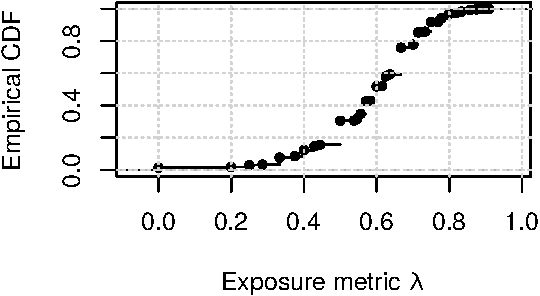
\includegraphics[width=0.75\linewidth]{figures/dns-exposure.pdf}
	\caption{Our AS exposure metric $\lambda$ for Alexa's Top 1,000 web sites.
	For half of all sites, 70\% of ASs are only traversed for DNS resolution,
	but not for subsequent web traffic.}
	\label{fig:exposure}
\end{figure}

\subsection{Mapping DNS resolvers}
\label{sec:mapping-resolvers}
Having shown that the Internet provides fertile ground for DNS-snooping
adversaries, let us now investigate how this affects the Tor network.  Key to
this question is an understanding of what DNS resolvers exit relays use.  Until
now, we only had anecdotal evidence, e.g., from OpenDNS-powered error messages
that some exit relays would occasionally show.

We identify the DNS resolver of all exit relays by using
exitmap~\cite{exitmap}, a scanner for Tor exit relays.  Exitmap automates
running a task---e.g., fetch a web page---over all one thousand exit relays,
making it possible to see the Internet through the ``eyes'' of every single
exit relay.  Leveraging exitmap, we resolve unique, relay-specific domains over
each exit relay, to a DNS server under our control.  This experiment is
visualized in Figure~\ref{fig:dnsenum}.  To improve reliability, we configured
exitmap to use two-hop circuits instead of the standard three-hop circuits.
The first hop was a guard relay under our control.  Over each exit relay, we
resolved a unique domain PREFIX.tor.nymity.ch.  The prefix consisted of the
relay's unique 160-bit fingerprint, concatenated to a random 40-bit string
whose purpose is to prevent caching, so exit relays indeed resolve each query
instead of responding with a cached element.  We controlled the authoritative
DNS server of tor.nymity.ch, so we could capture both the IP address and packet
content of every single query for tor.nymity.ch.

\begin{figure}[t]
	\centering
	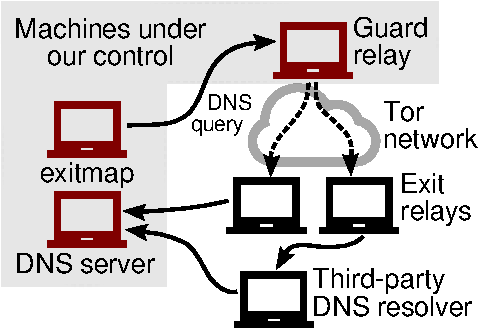
\includegraphics[width=0.65\linewidth]{figures/resolver-identification.pdf}
	\caption{Our method to identify the DNS resolvers of exit relays.  Over
	each exit relay, we resolve relay-specific domain names that are under our
	control.  Inspecting our DNS server logs, we can then identify the IP
	address of all exit relay resolvers.}
	\label{fig:dnsenum}
\end{figure}

An exit relay can either run its own resolver (see the left exit relay in
Figure~\ref{fig:dnsenum}), or use a third-party resolver such as the one
provided by its ISP (see the right exit relay in Figure~\ref{fig:dnsenum}).  If
an exit relay runs its own resolver, we expect to receive a DNS request from
the exit relay's IP address, but if an exit relay uses a third-party resolver,
we expect to receive a request from an unrelated IP address.  Having encoded
relay-specific fingerprints in the query names, we are able to map queries to
exit relays in such cases.  We ran this experiment from September 2015 to May
2016, at least once a day.  Once we started to analyze our data, we identified
the following two difficulties.

\paragraph{DNS proxies}
Manual inspection of our data revealed that several exit relays used DNS
proxies, i.e., machines that passed on DNS requests to an actual resolver
instead of resolving it themselves.  Google's resolver 8.8.8.8 is a popular
example of a DNS proxy; the actual resolution is documented to be done by
several dozen machines in the background~\cite{google-proxies}.  DNS proxies do
not interfere with our measurements, which is why we ignored them.

\paragraph{Multiple DNS resolvers}
On Linux systems, DNS resolution is controlled by the file
\texttt{/etc/resolv.conf}.  It contains a list of up to three DNS resolvers
that are queried in order.  If the primary resolver does not respond within a
time limit, the system falls back to the second, and finally the third
resolver, if available.  Our data suggests that several exit relays used
different resolvers in subsequent exitmap scans---one relay, for example, used
both Google's DNS resolver and one provided by its ISP.  For our visualization,
we only consider the first resolver we observed for an exit relay, which might
not be the primary resolver.  

\subsubsection{Visualizing results}
Figure~\ref{fig:exit-resolvers} illustrates the fraction of DNS requests that
all ASs that were ever in the top three could observe.  Google averages at
33\%, but at times saw more than 40\% of all DNS requests exiting the Tor
network---an alarming number for a single organization.  Second to Google is
``Local,'' i.e., exit relays that run their own resolver, averaging at 12\%.
Next is OVH which used to be as popular as local resolvers, but slowly lost its
share over time.  Note that in contrast to Google, OVH does not run a public
DNS server; the company's resolvers are only accessible to its customers.
Between 0\% and 5\% are seven more ASs, labeled as ``Others,'' namely Level 3,
Visual Online, Init7, OpenDNS, Cyberdyne, NForce, and LeaseWeb.  Apart from the
illustrated top resolvers, the distribution has a long tail, presumably
consisting of many ISP resolvers.

\begin{figure*}[t]
	\centering
	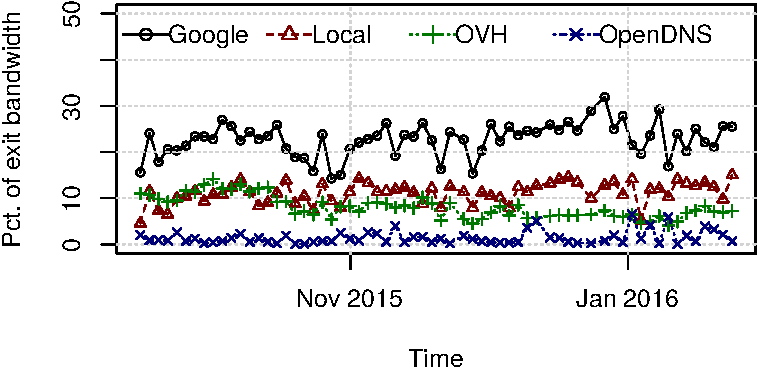
\includegraphics[width=\linewidth]{figures/exit-resolvers.pdf}
	\caption{The amount of the most popular DNS resolvers of exit relays over
		time, weighted by bandwidth.  Google's DNS server is by far the most
		popular resolver of exit relays, followed by a local resolver, OVH, and
		OpenDNS.  The category ``Other'' consists of the ASs Level 3, Visual
		Online, Init7, OpenDNS, Cyberdyne, NForce, and LeaseWeb.}
	\label{fig:exit-resolvers}
\end{figure*}

% The following section takes up too much space, so it's commented out for now.
% We should include it in an extended version of our work, though.
\iffalse
\subsection{Mapping resolver configuration}
\label{sec:mapping-configuration}
In addition to identifying an exit relay's DNS resolver, our technique can
ascertain parts of its configuration.  Resolvers with poor or broken
configuration pose a security risk to Tor users as attackers could poison or
enumerate their cache, allowing them to redirect users or profile them.
Therefore, it is important to identify broken resolvers because they jeopardize
the anonymity of Tor users.

\paragraph{Random source ports}
To impede cache poisoning attacks, DNS resolvers should use random source ports
instead of always using UDP port 53.  Our data allows for verifying if a given
resolver randomizes its source ports.  We classify a resolver as ``uses
randomization'' if the source port does not equal 53.  Note that this method
causes a small number of false positives because a randomizing resolver could
use port 53 simply by chance.  However, the probability of that happening is
only $\frac{1}{65535}$.

We found 135 DNS resolvers that did not use random source ports.  These
resolvers were located in the networks of Vodafone, Germany (95\%), MTNL, India
(4\%), and Cogent, U.S. (1\%).

\paragraph{0x20 encoding}
Resolvers can further reduce the chance of cache poisoning by employing 0x20
encoding, i.e., randomizing the capitalization of domain names.  For example,
to resolve foo.com, a resolver would send a request for fOo.CoM.  If the DNS
response does not reflect the randomly chosen capitalization, the resolver
considers unauthentic.  We classify a resolver as ``uses 0x20'' if it has at
least one lowercase and one uppercase character.  Again, there is a chance of
false positives, which depends on the domain name length.  A 0x20-encoded
domain name of $n$ characters (excluding periods) can be all-uppercase or
all-lowercase with probability $2 \cdot 0.5^n$.

We found 427 DNS resolvers that did not use 0x20 encoding for at least one
query.  The top five resolvers were located in the networks of Google, U.S.
(38\%), AT\&T, U.S. (22\%), Deutsche Telekom, Germany (7\%), Yandex, Russia
(7\%), OpenDNS, U.S. (4\%).

\paragraph{DNSSEC validation}
We can verify if a resolver is validating DNSSEC-signed records by resolving a
domain whose signature is deliberately malformed.  Such a service is provided
by dnssec-failed.org.  A validating resolver would not return an A record while
a non-validating resolver would.  Therefore, we resolve dnssec-failed.org over
all exit relays and check if we get an A record in response.
\fi
